% ##################################################################################################################
\section{Trondheim}
\label{sec:trondheim}
\hfill \textbf{Authors:} Stefan Flügel, Julia Kern, Frederik Bockemühl

\editdone{This text has undergone the professional edit. Please no grammatical changes anymore! They are most-probably wrong.}

% ##################################################################################################################
The Institute of Transport Economics (TØI), in cooperation with Julia Kern from TU-Berlin and Frederik Bockemühl from Hasselts University, built a first prototype model for the region of Trondheim (Norway) \citep[][]{FluegelKern_unpub_WTS_2014}.

The road network data was imported from a publicly accessible data base (Elveg). Figure~\ref{fig:trondheimnetwork} illustrates the network. 
%
\createfigure%
{Network and simulated traffic in Trondheim and surroundings}%
{Network and simulated traffic in Trondheim and surroundings for 6:55\,am \citep[source][]{FluegelEtAl_Samferdsel_2014}}%
{\label{fig:trondheimnetwork}}%
{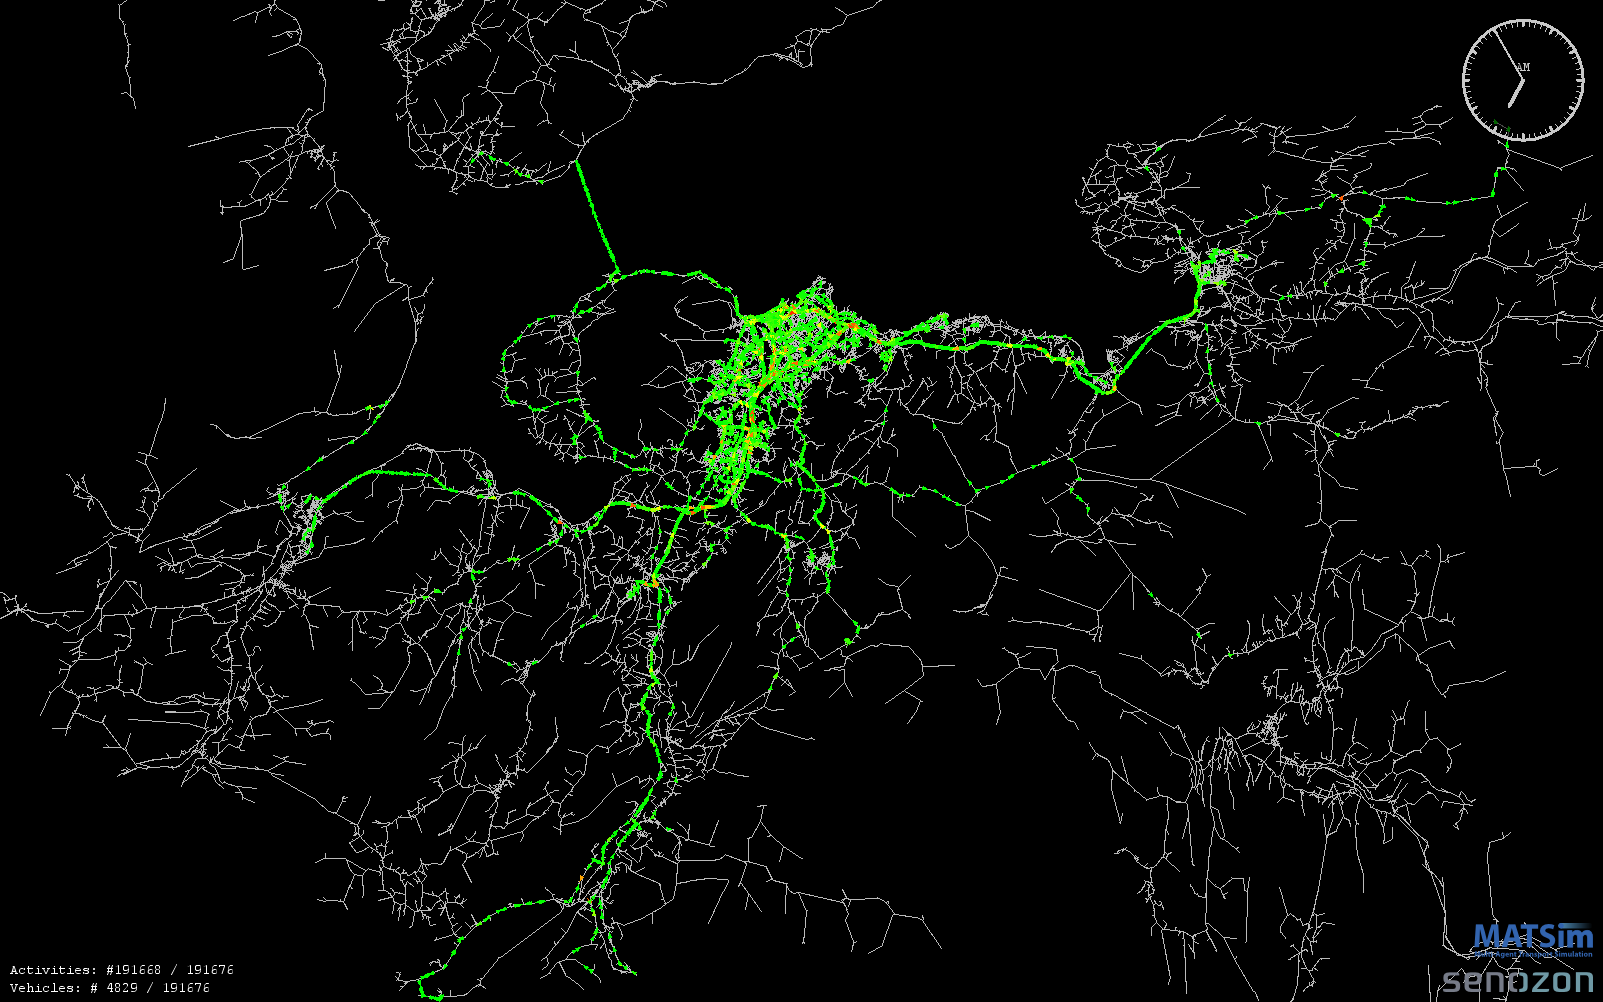
\includegraphics[width=0.85\textwidth, angle=0]{./using/figures/trondheimnetwork.png}}%
{}
%
Most required link information could be directly inferred from the data base. The lane capacity (vehicles per hour) was assumed to be a flat 1\,800 per lane. Existing toll stations, with their current toll structures, were coded manually in the network file. The public transport, walk and cycle networks had not been implemented at this time. Agents using one of these modes were teleported; travel times were calculated with predefined speeds per transport mode. 
Initial demand was derived from the National Travel Survey (NTS 2009) travel diaries. 4\,453 respondents were simply scaled up to 191\,676 agents; activity locations and departure times were slightly randomized to avoid clusters. This model differentiated only between work and "other" activities. Desirable working hours were specified as 8\,hours; demand consisted only of private cars (no trucks). 

Standard utility functions were applied, but in the calibration process, default values for travel time disutility in different transport modes were adjusted so that the model would reproduce observed market shares. The simulated traffic fit (in the reference scenario) against real-world counts was deemed satisfactory for a first implementation \citep[][]{Bockemuehl_TechRep_UH_2014}. 

Standard behavioral modules in \gls{matsim} were included in the Trondheim model. Agent could react to policy measures through three choice dimensions: changing route, changing transport mode and changing departure time. To test whether \gls{matsim} predicted reasonable behavioral changes, a small case study was performed. Additional tolls on streets (bridges and tunnels) to Trondheim city center were coded in the network and three congestion price structure were tested. Figure~\ref{fig:loadcurve} illustrates the effects on the simulated cars entering and leaving Trondheim city center. 
%
\createfigure%
{Cars entering/leaving Trondheim city center}%
{Cars entering/leaving Trondheim city center in reference scenario and three congestion pricing scenarios \citep[source][]{Bockemuehl_TechRep_UH_2014}}%
{\label{fig:loadcurve}}%
{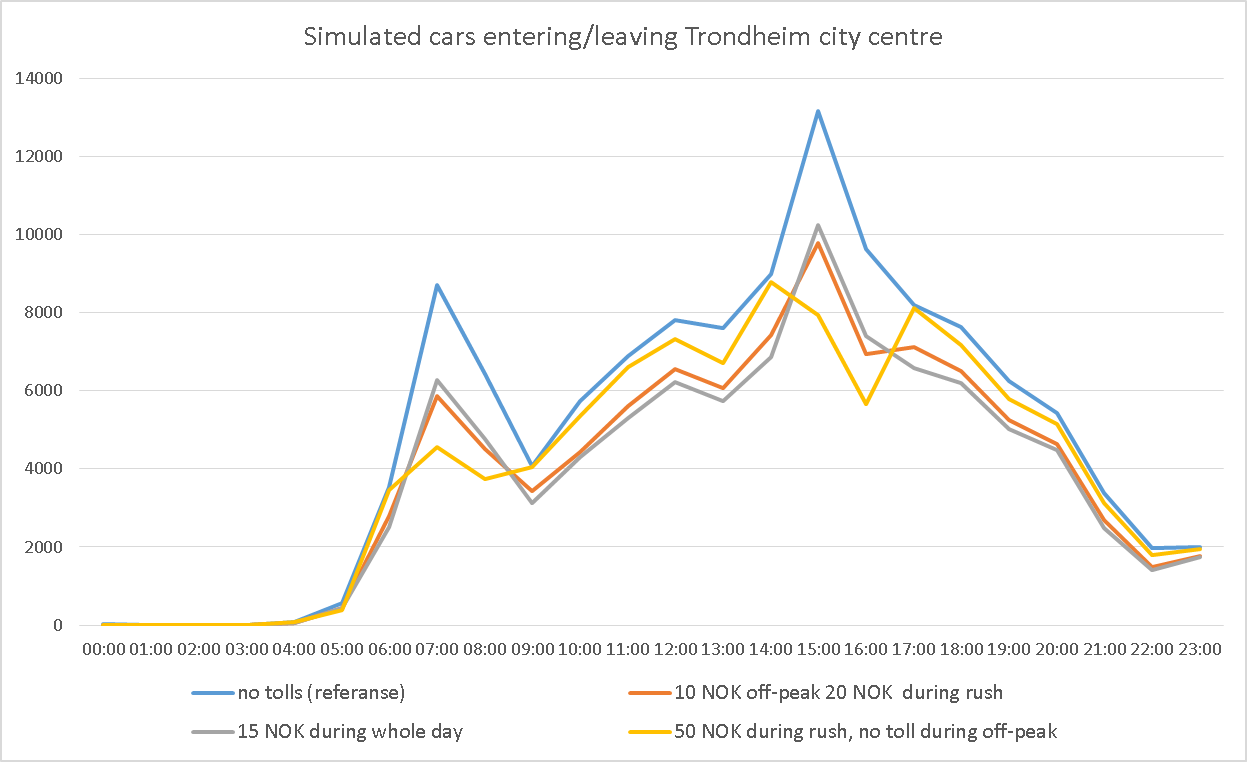
\includegraphics[width=0.85\textwidth, angle=0]{./using/figures/trondheimloadcurve.png}}%
{}
%
Compared to the reference scenario without tolls, total number of cars was reduced in all toll scenarios. Some agents changed transport modes; others, who would have driven through Trondheim center, changed their route. Comparing the three different congestion-pricing structures, it was also evident that agents changed departure time. The difference between the 15\,\glspl{nok} flat scenario and the 10/20\,\glspl{nok} scenario was small; the effect in the 50\,\glspl{nok} rush scenario was substantial. Actually, in this scenario, traffic was heavier before 3\,pm and after 5\,pm implying that many agents changed departure time to avoid high congestion pricing.  

% ##################################################################################################################   










